\section{Design}
Conceptualizing a single ETL process as an entity of type \textit{Task}, that is, the ``extraction, transformation and loading of data from a source to destination'', provides a focal point on which the nETL software can be architected. Handling of instances of type \textit{Task} is done by an entity of type \textit{TaskManager}, which for the purposes of nETL v1.0 is implemented as a singleton (many instances of \textit{TaskManager} could potentially be useful if scaling of nETL were required). Objects of type \textit{Task} are instantiated via a \textit{Task} constructor, which takes a configuration object as an argument. This configuration is specified as a JSON file in which an operation of type \textit{Extraction}, operation(s) of type \textit{Transformation} and an operation of type \textit{Load} is described as sub-objects within the JSON file.

Starting the long-running nETL process comprises instantiating the \mintinline{text}{taskManager} singleton. This object provides a CLI (command line interface) to facilitate user interactions. Via the CLI, users can interact with \mintinline{text}{taskManager} to load components, start/stop tasks, configure application options such as log output path, etc.

\begin{figure}[H]
    \centering
    \begin{mdframed}
        \centering
        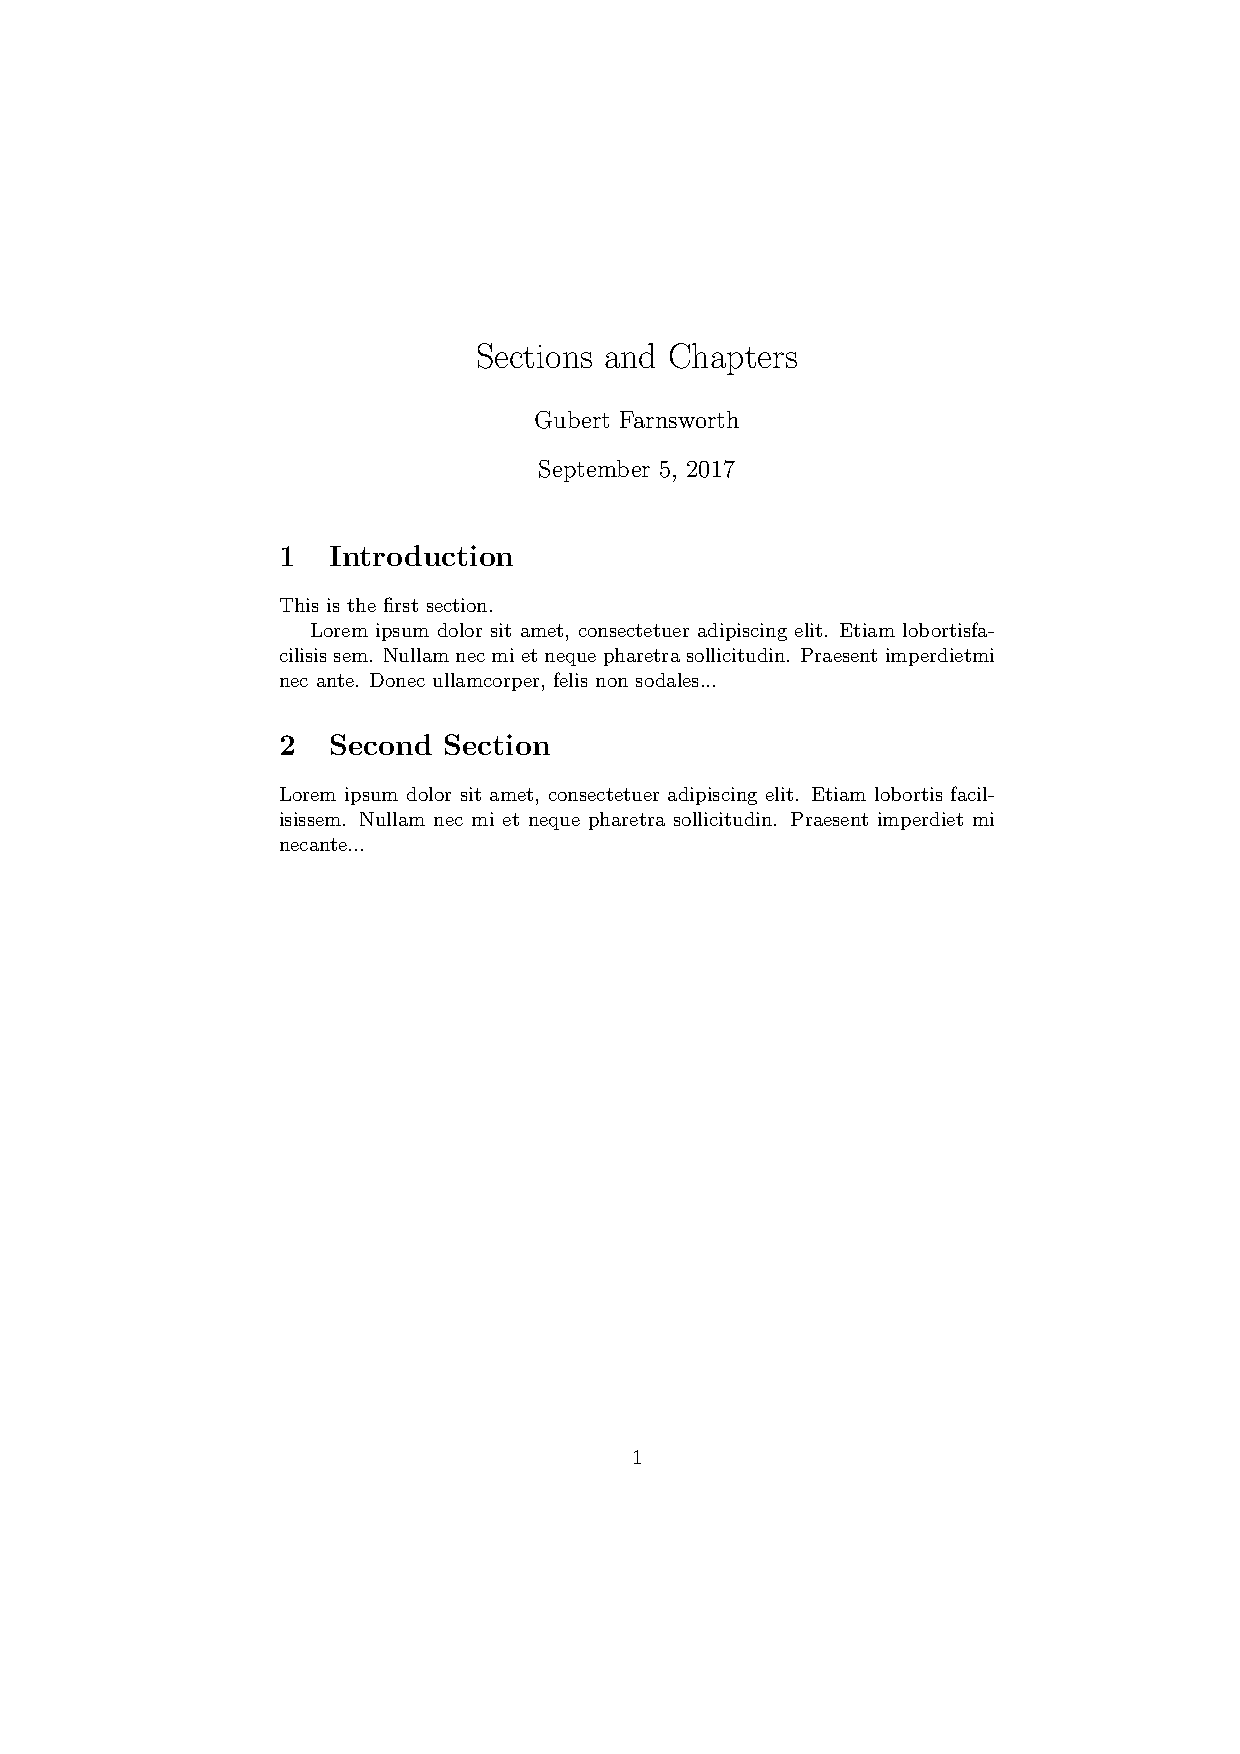
\includegraphics[scale=0.39]{./resources/figures/netl.png}
    \end{mdframed}
    \caption[nETL Architecture]{\textbf{Figure \ref{nETL}: nETL Architecture.} \textit{nETL} is an ETL framework designed to host user-created \textit{Modules} to define \textit{extraction}, \textit{transformation} and \textit{loading} processes. \textit{Modules}, shown in the colored boxes, consist of two parts: a configuration object (a JSON object) and a function that adheres to the specified contract. On startup the \textit{nETL} framework loads modules via the operations via a function made available by the main class. The modules are then cached in main memory by the \textit{nETL} process. A user can then interact with the TaskManager class to create a new task via loading a JSON configuration that makes use of a particular \textit{Module}. Tasks consist of an \textit{Extraction module} configuration, several \textit{Transformation module} configurations and a \textit{Load} configuration. Because modules are created and defined by users, as well as the order in which modules are executed, input/output contracts are also defined by the user, and as such \textit{ETL} processes are infinitely configurable.}
    \label{nETL}
\end{figure}

Figure \ref{fig-nETL} shows the architecture for the nETL application - a configurable component-based ETL tool structured as a framework in which modules can be written for extraction, transformation and load \textit{tasks}. Module components are shown in the shaded boxes in the diagram and consist of two things: a configuration object specified in JSON format, and a JavaScript module that adheres to the specified contract format. References to tasks are created by module instantiation, which the contract stipulates should return an object with two properties: \mintinline{text}{name} and \mintinline{text}{exe}. The main \mintinline{text}{Application} singleton references the \mintinline{text}{exe} property of each module using the \mintinline{text}{name} value returned. the \mintinline{text}{exe} property references a function that is executed when a task specifies a particular module as part of the task's processing.

On task-module execution, the function referenced via \mintinline{text}{exe} returns a function with a specified method name: \mintinline{text}{getNext()} for extractions, \mintinline{text}{transform(Object: obj)} for transformation, \mintinline{text}{batch(List: data)}. These methods are called in order during task execution - \mintinline{text}{getNext()} is called once per batch, \mintinline{text}{transform(obj)} is called once per item in each batch, and \mintinline{text}{load()} is called once per batch - until all data has been processed. The \mintinline{text}{Application} singleton controls reference-scoping during task execution, as well as providing an engine that serializes and controls task execution from start to finish. Part of this functionality includes error handling, logging, state persistence, and an API for user-process communication. Users can use the command line API to interact with \mintinline{text}{Application} to load task-modules, and with \mintinline{text}{taskManager} to load task-configurations. This architecture allows for separation of concerns; modules are self-contained and user-defined, as are the order in which these modules are executed (according to task configuration files). As such nETL allows for infinitely configurable data-flow processes.

\begin{itemize}
    \item It has a very succinct API making it fast to write code in (i.e. it is a highly abstracted language similarly to Ruby or Python)
    \item But unlike Ruby or Python (and other high level languages), it is opinionated in that it handles IO asynchronously by default
    \item The JavaScript implementation of object-orientation is appealing (to some developers at least \cite{jsBook})
    \item JavaScript is very much in line with the spirit of CouchDB
\end{itemize}